\section{ESP32 a jeho programátor}


\begin{wrapfigure}{L}{0.4\textwidth}
    \centering
    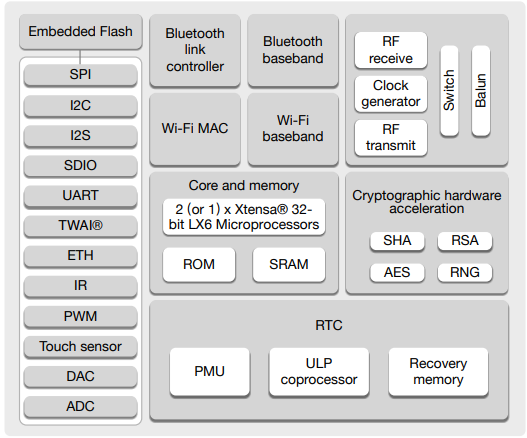
\includegraphics[width=0.4\textwidth]{kapitoly/obrazky/E4/ESP32/BlockDiagram.png}
    \caption{\label{fig:E4-ESP32-BlockDiagram}Zapínání a ochrana proti přepólovaní}
\end{wrapfigure}

Mozkem celého trezoru je~čip~\href{https://www.espressif.com/sites/default/files/documentation/esp32-wrover-b_datasheet_en.pdf}{ESP32-wrover}. 
Obsahuje dva dvaatřicetibitové procesory Xtensa LX6 taktované až~na~240Mhz. ESP32 má také na modulu wrover k dispozici 520 KiB SRAM 
a~4,8 nebo 16~Mb flash paměti. ESP32 má také k~dispozici řadu periferií, z~nichž asi nejvýznamnější je WiFi a~Bluetooth. Právě integrace 
WiFi a~Bluetoothu je také jeden z~primárních důvodů volby tohoto čipu. Dalším podstatným důvodem volby čipu ESP32 je jeho vysoký výpočetní výkon, 
alespoň na poměry mikrokontrolérů a~v~neposlední řadě také fakt, že s~tímto čipem už nějakou dobu pracuji a~tak ho již znám. Konkrétně wrover 
jsem pak zvolil kvůli dodatečné paměti PSRAM (Pseudo Static RAM), \href{http://gamma.spb.ru/images/pdf/esp-psram32_datasheet_en.pdf}{ESP-PSRAM32}.

%todo čiste pro info - jak je velká? 

\begin{figure}[htbp] %todo do přílohy 
    \centering
    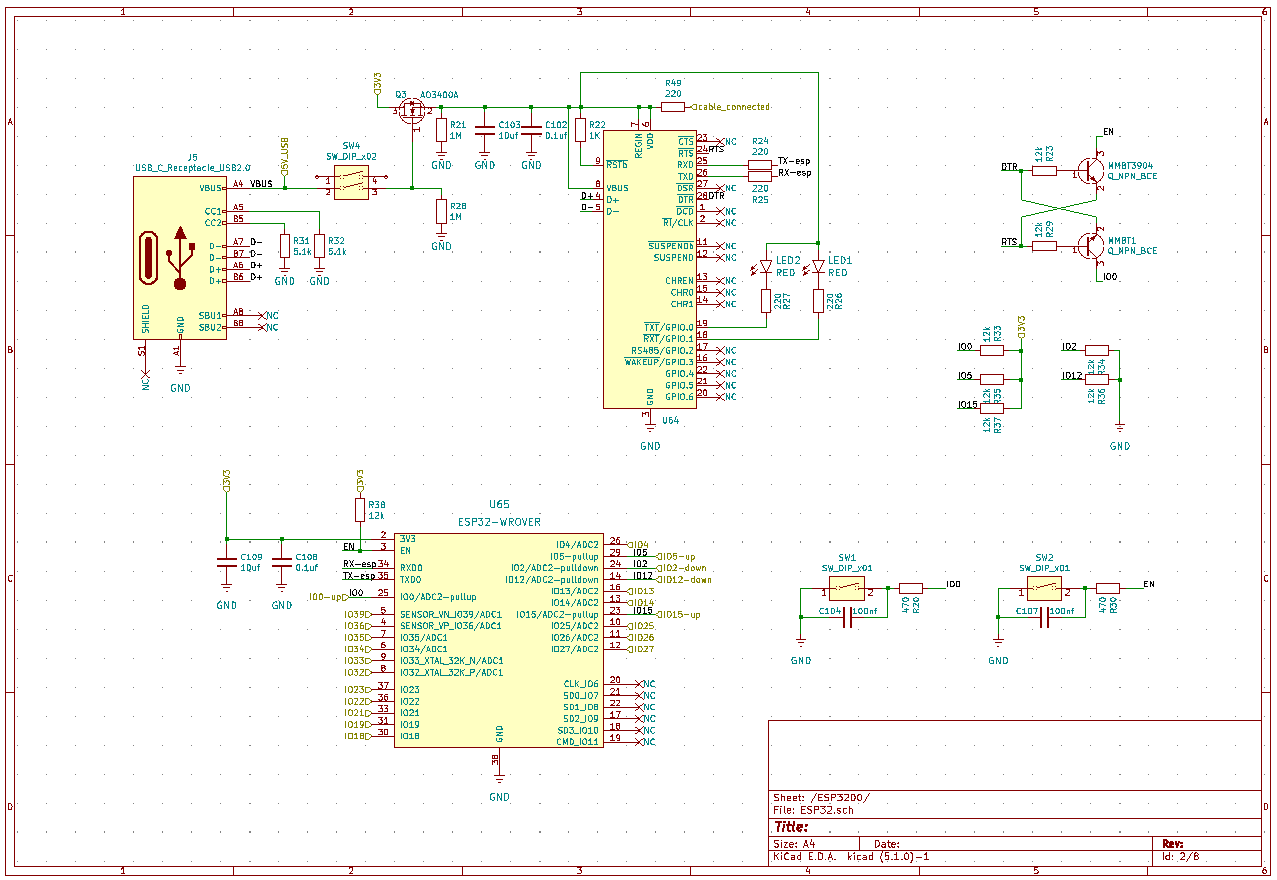
\includegraphics[width=\textwidth]{kapitoly/obrazky/E4/ESP32/sch.png}
    \caption{Zapojení ESP32}
    \label{fig:E4-step-up}
\end{figure}

ESP32 také vyžaduje mít při startu definované úrovně na některých pinech, proto jsou zde čtyři pull-upy a dva pull-downy, které definují výchozí stav
pinů IO0, IO2, IO12, IO15 a EN.  %todo pinů je 5 a rezistorů 6? na co 4 pull-up? 
\begin{table}[h]
    \centering
    \resizebox{\textwidth}{!}{%
    \begin{tabular}{l|l|l}\midrule
    \textbf{IO0}    & ovládá boot procesoru             & LOW při resetu ESP vstupuje do bootloaderu    \\\midrule
    \textbf{IO2}    & potvrzení pro spuštění bootu      & LOW potvrzuje                                 \\\midrule
    \textbf{IO12}   & určuje napětí komunikace s flash  & LOW znamená napětí 3,3V a HIGH 1,8V           \\\midrule
    \textbf{IO15}   & ovládá zprávy bootloaderu do UART & LOW zprávy vypíná a HIGH zapíná               \\\midrule
    \textbf{EN}     & reset pin                         & LOW ESP je drženo v resetu                    \\\midrule
    \end{tabular}%
    }
    \caption{Popis funkce pinů}
    \label{tab:COMPARATION}
\end{table}

\newpage

\subsection*{Programátor}
Aby mohl uživatel trezor jednoduše naprogramovat, je~na~desce převodník USB-UART, \href{https://www.silabs.com/documents/public/data-sheets/cp2102n-datasheet.pdf}{CP2102}.
Protože však CP2102 není potřeba celou dobu provozu a~protože trezor nemá k~dispozici neomezený zdroj elektřiny, je~převodník zapnut jen ve~chvíli, 
kdy je~připojeno USB-C, které slouží jak pro nabíjení, tak pro programování. Vypínání převodníku je zajištěno tranzistorem Q3, který je zároveň společně
s~DIP~switchem SW4 využit pro možnost zákazu programování, zapojení přikládám na obrázku \ref{fig:E4-sch_ESP32}.

\newpage